% Q9: preserve the four qualitative alternatives from the fixed scan.
% Curve scales are schematic; only axes, orientations, and opening directions matter.
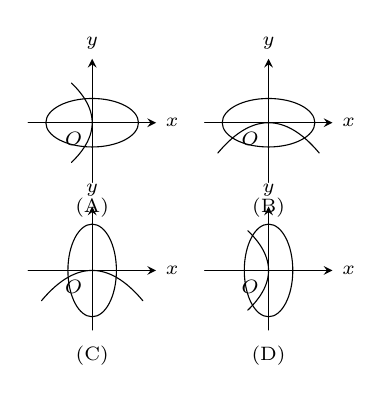
\begin{tikzpicture}[
  x=0.56cm,y=0.56cm,line cap=round,line join=round,>=stealth,
  every node/.style={font=\scriptsize}
]
\def\axes{%
  \draw[->] (-1.45,0)--(1.45,0) node[right] {$x$};
  \draw[->] (0,-1.35)--(0,1.45) node[above] {$y$};
  \node[below left] at (0,0) {$O$};
}
\def\leftparabola{%
  \draw[domain=-0.9:0.9,samples=60,variable=\t]
    plot ({-0.58*\t*\t},{\t});
}
\def\downparabola{%
  \draw[domain=-1.15:1.15,samples=60,variable=\t]
    plot ({\t},{-0.52*\t*\t});
}
\begin{scope}[shift={(0,0)}]
  \axes
  \draw (0,0) ellipse [x radius=1.05,y radius=0.55];
  \leftparabola
  \node[below] at (0,-1.48) {(A)};
\end{scope}
\begin{scope}[shift={(4,0)}]
  \axes
  \draw (0,0) ellipse [x radius=1.05,y radius=0.55];
  \downparabola
  \node[below] at (0,-1.48) {(B)};
\end{scope}
\begin{scope}[shift={(0,-3.35)}]
  \axes
  \draw (0,0) ellipse [x radius=0.55,y radius=1.05];
  \downparabola
  \node[below] at (0,-1.48) {(C)};
\end{scope}
\begin{scope}[shift={(4,-3.35)}]
  \axes
  \draw (0,0) ellipse [x radius=0.55,y radius=1.05];
  \leftparabola
  \node[below] at (0,-1.48) {(D)};
\end{scope}
\end{tikzpicture}
